\subsection[Relationship between ozone, NOx and Temperature]{Relationship between Ozone, \ce{NO_x} and Temperature} \label{ss:r_contours} 
\begin{figure}%
    \centering%
    \caption{Contours of peak ozone mixing ratios (ppbv) as a function of the total \ce{NO_x} emissions and temperature for each chemical mechanism using a temperature-dependent and temperature-independent source of isoprene emissions. The contours can be split into three separate regimes: High-\ce{NO_x}, Maximal-\ce{O3} and Low-\ce{NO_x} indicated in the figure.}
    \label{f:ozone_contours}%
    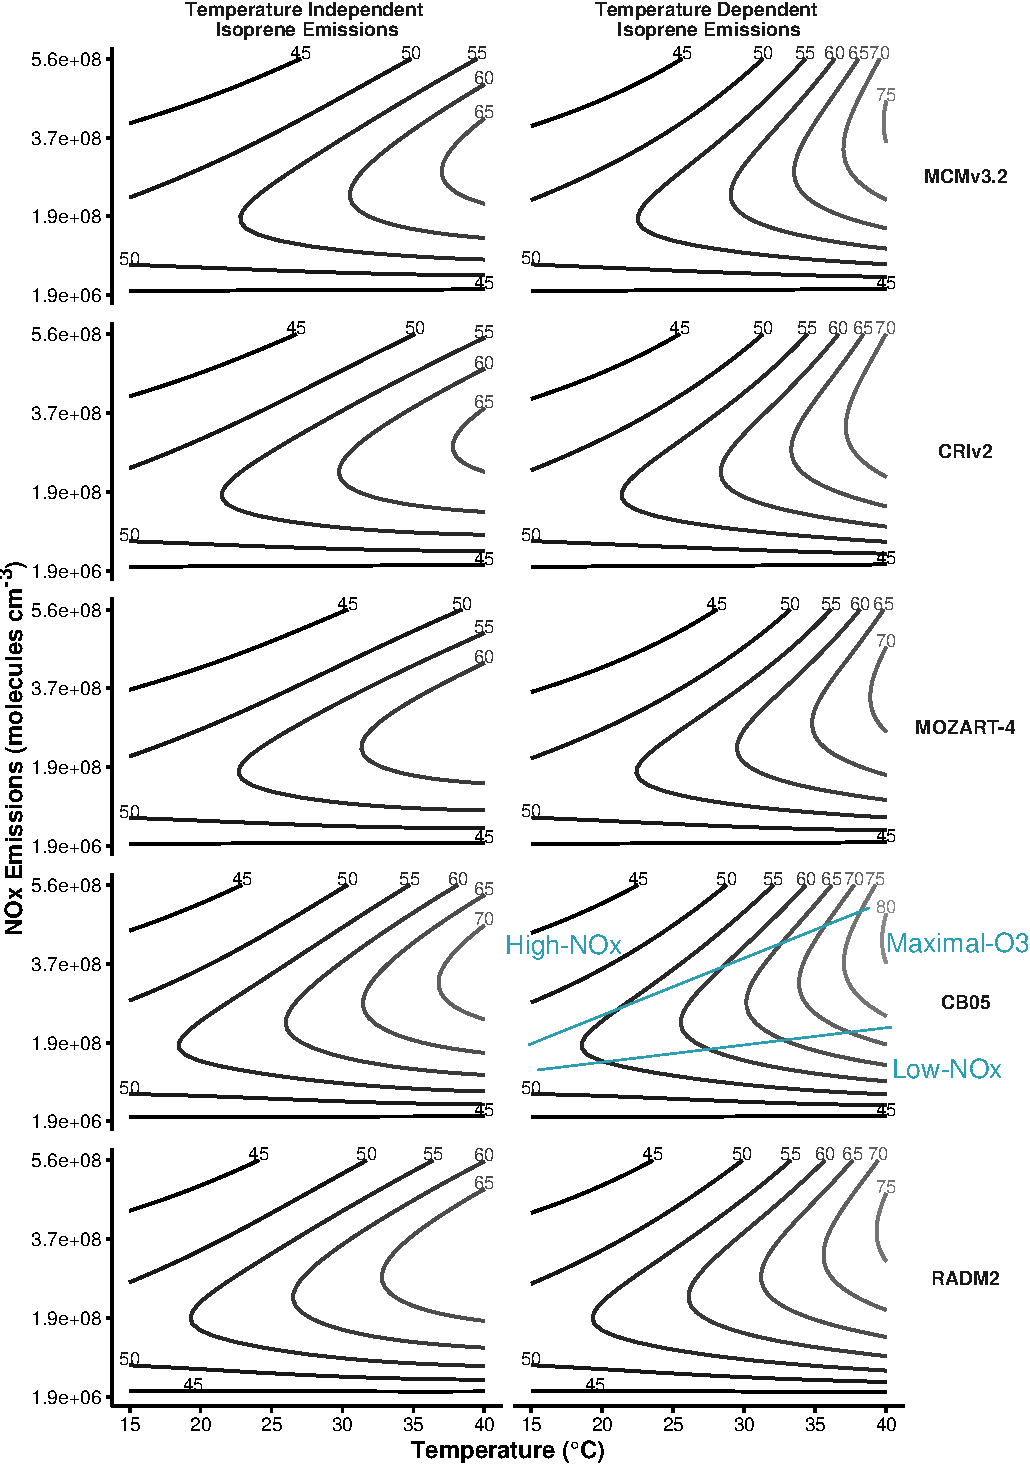
\includegraphics[width=\textwidth]{img/O3_comparison}%
\end{figure}

\begin{figure}[t]%
    \centering%
    \caption{Mean ozone mixing ratios (ppbv) at each temperature after allocation to the different \ce{NO_x}-regimes of Fig.~\ref{f:ozone_contours}. The differences in ozone mixing ratios due to chemistry (solid line) and isoprene emissions (dotted line) are represented graphically for MOZART-4 with High-\ce{NO_x} conditions. Table~\ref{t:differences} details the differences for each chemical mechanism and \ce{NO_x}-condition.}%
    \label{f:O3-T}%
    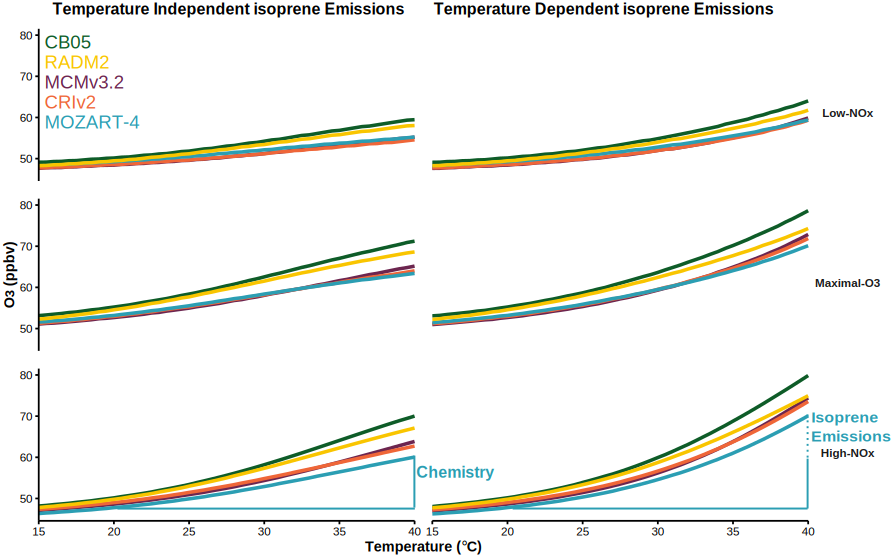
\includegraphics[width=\textwidth]{img/O3-T_correlation}%
    \vspace{-4mm}
\end{figure}

\begin{table}[t]%
    \centering%
    \caption{Increase in mean ozone mixing ratio (ppbv) due to chemistry (i.e. faster reaction rates) and temperature-dependent isoprene emissions from $20$~\degree C to $40$~\degree C in the \ce{NO_x}-regimes of Fig.~\ref{f:O3-T}.}%
    \label{t:differences}%
    \begin{tabularx}{\textwidth}{c|c *{3}{|c}} 
    \hline \hline
    \textbf{Chemical} & \textbf{Source of} & \multicolumn{3}{c}{\textbf{Increase in Ozone from 20~$^{\circ}$C to 40~$^{\circ}$C (ppbv)}} \\ \cline{3-5}
    \textbf{Mechanism} & \textbf{Difference} & \textbf{Low-\chem{NO_x}} & \textbf{Maximal-\chem{O_3}} & \textbf{High-\chem{NO_x}} \\ 
    \hline \hline
    \multirow{2}{*}{MCMv3.2} & Isoprene Emissions & 4.6 & 7.7 & 10.6 \\ 
    & Chemistry & 6.8 & 12.5 & 15.2 \\ \hline
    \multirow{2}{*}{CRIv2} & Isoprene Emissions & 4.8 & 7.9 & 10.8 \\
    & Chemistry & 6.0 & 11.1 & 13.7 \\ \hline
    \multirow{2}{*}{MOZART-4} & Isoprene Emissions & 4.1 & 6.7 & 10.0 \\
    & Chemistry & 6.0 & 10.2 & 12.3 \\ \hline
    \multirow{2}{*}{CB05} & Isoprene Emissions & 4.6 & 7.4 & 9.8 \\
    & Chemistry & 9.3 & 16.0 & 19.9 \\ \hline
    \multirow{2}{*}{RADM2} & Isoprene Emissions & 3.8 & 5.7 & 7.8 \\ 
    & Chemistry & 8.6 & 14.1 & 17.3 \\
    \hline \hline
\end{tabularx}
%
    \vspace{-4mm}
\end{table}

Figure~\ref{f:ozone_contours} depicts the peak mixing ratio from ozone of each simulation as a function of the total \ce{NO_x} emissions and temperature when using a temperature-independent and temperature-dependent source of isoprene emissions for each chemical mechanism.
A non-linear relationship of ozone mixing ratios with \ce{NO_x} and temperature is produced by each chemical mechanism.
This non-linear relationship is similar to that determined by \citet{Pusede:2014} using an analytical model constrained to observational measurements over the San Joaquin Valley, California.

Higher peak ozone mixing ratios are produced when using a temperature-dependent source of isoprene emissions (Fig.~\ref{f:ozone_contours}).
The highest mixing ratios of peak ozone are produced at high temperatures and moderate emissions of \ce{NO_x} regardless of the temperature dependence of isoprene emissions.
Conversely, the least amount of peak ozone is produced with low emissions of \ce{NO_x} over the whole temperature range ($15$ -- $40$~\degree C) when using both a temperature-independent and temperature-dependent source of isoprene emissions.

The contours of ozone mixing ratios as a function of \ce{NO_x} and temperature can be split into three \ce{NO_x} regimes (Low-\ce{NO_x}, Maximal-\ce{O3} and High-\ce{NO_x}), similar to the \ce{NO_x} regimes defined for the non-linear relationship of ozone with VOC and \ce{NO_x}.
The Low-\ce{NO_x} regime corresponds with regions having little increase in ozone with temperature, also called the \ce{NO_x}-sensitive regime.
The High-\ce{NO_x} (or \ce{NO_x}-saturated) regime is when ozone levels increase rapidly with temperature. 
The contour ridges correspond to regions of maximal ozone production; this is the Maximal-\ce{O3} regime.
\citet{Pusede:2014} showed that temperature can be used as a proxy for VOC, thus we assigned the ozone mixing ratios from each box model simulation to a \ce{NO_x} regime based on the \ce{H2O2}:\ce{HNO3} ratio.
This ratio was used by \citet{Sillman:1995} to designate ozone to \ce{NO_x} regimes based on \ce{NO_x} and VOC levels. 
The Low-\ce{NO_x} regime corresponds to \ce{H2O2}:\ce{HNO3} ratios less than $0.5$, the High-\ce{NO_x} regime corresponds to ratios larger than $0.3$ and ratios between $0.3$ and $0.5$ correspond to the Maximal-O3 regime.

The peak ozone mixing ratio from each simulation was assigned to a \ce{NO_x} regime based on the \ce{H2O2}:\ce{HNO3} ratio of that simulation.
The peak ozone mixing ratios assigned to each \ce{NO_x} regime at each temperature were averaged, and illustrated in Fig.~\ref{f:O3-T} for each chemical mechanism and each type of isoprene emissions (temperature independent and temperature dependent).  
We define the absolute increase in ozone from $20$~\degree C to $40$~\degree C due to faster reaction rates as the difference between ozone mixing ratios from $20$~\degree C to $40$~\degree C when using a temperature-independent source of isoprene emissions.
When using a temperature-dependent source of isoprene emissions, the difference in ozone mixing ratios from $20$~\degree C to $40$~\degree C minus the increase due to faster reaction rates, gives the absolute increase in ozone mixing ratios from increased isoprene emissions.
These differences are represented graphically in Fig.~\ref{f:O3-T} and summarised in Table~\ref{t:differences}.

Table~\ref{t:differences} shows that the absolute increase in ozone with temperature due to chemistry (i.e.~faster reaction rates) is larger than the absolute increase in ozone due to increased isoprene emissions for each chemical mechanism and each \ce{NO_x} regime.
In all cases the absolute increase in ozone with temperature is largest under High-\ce{NO_x} conditions and lowest with Low-\ce{NO_x} conditions (Fig.~\ref{f:O3-T} and Table~\ref{t:differences}).
The increase in ozone mixing ratio from $20$~\degree C to $40$~\degree C due to faster reaction rates with High-\ce{NO_x} conditions is almost double that with Low-\ce{NO_x} conditions.  
In the Low-\ce{NO_x} regime, the increase of ozone with temperature using the reduced chemical mechanisms (CRIv2, MOZART-4, CB05 and RADM2) is similar to that from the MCMv3.2. 
Larger differences occur in the Maximal-\ce{O3} and High-\ce{NO_x} regimes.

All reduced chemical mechanisms except RADM2 have similar increases in ozone due to increased isoprene emissions as the MCMv3.2 (Table~\ref{t:differences}).
RADM2 produces $3$~ppbv less ozone than the MCMv3.2 due to increased isoprene emissions in each \ce{NO_x} regime, indicating that this difference is due the representation of isoprene degradation chemistry in RADM2.

\citet{Coates:2015} compared ozone production in different chemical mechanisms to the MCMv3.2 using the TOPP metric (Tagged Ozone Production Potential) as defined in \citet{Butler:2011} and showed that less ozone is produced per molecule of isoprene emitted using RADM2 than with MCMv3.2.
The degradation of isoprene has been extensively studied and it is well-known that methyl vinyl ketone (MVK) and methacrolein are signatures of isoprene degradation \citep{Atkinson:2000}.
All chemical mechanisms in our study except RADM2 explicitly represent MVK and methacrolein (or in the case of CB05, a lumped species representing both these secondary degradation products).
RADM2 does not represent methacrolein and the mechanism species representing ketones (KET) is a mixture of acetone and methyl ethyl ketone (MEK) \citep{Stockwell:1990}. 
Thus the secondary degradation of isoprene in RADM2 is unable to represent the ozone production from the further degradation of the signature secondary degradation products of isoprene, MVK and methacrolein.
Updated versions of RADM2, RACM \citep{Stockwell:1997} and RACM2 \citep{Goliff:2013}, sequentially included methacrolein and MVK and with these updates the ozone production from isoprene oxidation approached that of the MCMv3.2 \citep{Coates:2015}.

\subsection{Ozone Production and Consumption Budgets} \label{ss:r_budgets}
\begin{figure}[t]%
    \centering%
    \caption{Day-time budgets of \ce{O_x} normalised by the total loss rate of emitted VOC in the \ce{NO_x}-regimes of Fig.~\ref{f:O3-T}. The white line indicates net production or consumption of \ce{O_x}. The net contribution of reactions to \ce{O_x} budgets are allocated to categories of inorganic reactions, peroxy nitrates (RO2NO2), reactions of NO with HO2, alkyl peroxy radicals (RO2) and acyl peroxy radicals (ARO2). All other reactions are allocated to the `Other Organic' category.}%
    \label{f:ozone_budgets}% 
    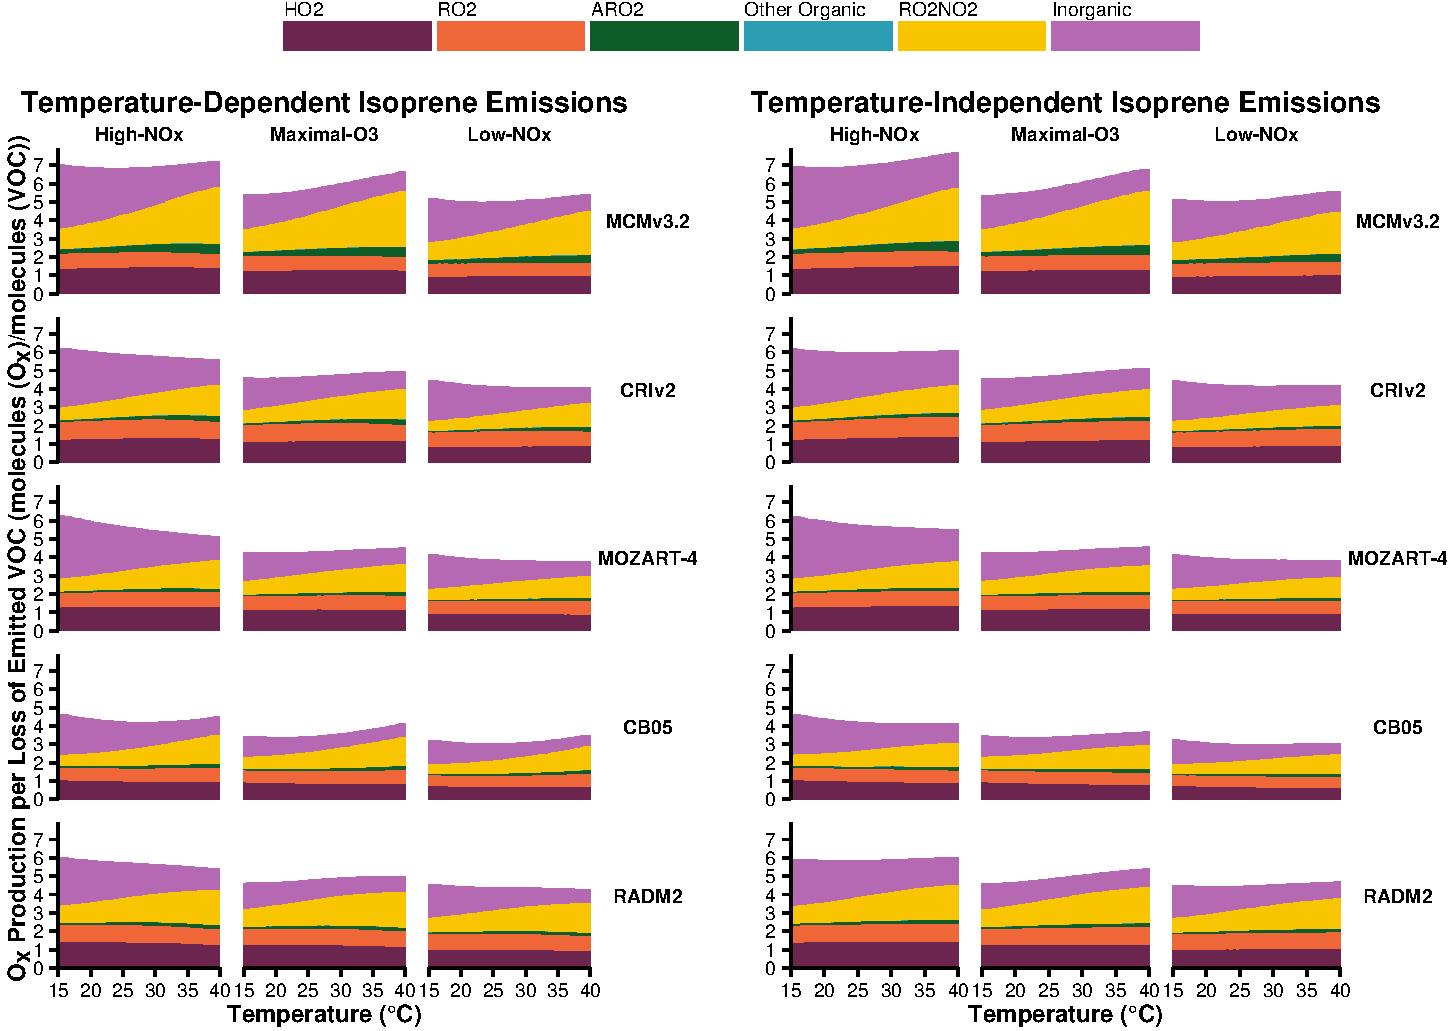
\includegraphics[width = \textwidth]{img/Ox_budgets}% 
    \vspace{-4mm}
\end{figure}
% 
In order to understand the temperature dependence of ozone production directly, we examine the modelled day-time production and consumption budgets of \ce{O_x} ($\equiv$ \ce{O3 + NO2 + O(^1D) + O}) normalised by the total chemical loss rate of the emitted VOC (Fig.~\ref{f:ozone_budgets}).
The \ce{O_x} budgets are assigned to each \ce{NO_x} regime for each chemical mechanism and type of isoprene emissions.
The budgets are allocated to the net contribution of major chemical categories, where `HO2', `RO2', `ARO2' represent the reactions of NO with \ce{HO2}, alkyl peroxy radicals and acyl peroxy radicals respectively.
`RO2NO2' represents the net effects of peroxy nitrates, which remove \ce{O_x} when produced and are a source of \ce{O_x} when they thermally decompose.
`Inorganic' is all other inorganic contributions to \ce{O_x} production and any other remaining organic reactions are included in the `Other Organic' category.
Figure~\ref{f:ozone_budgets} also illustrates the net production or consumption of \ce{O_x} in each case.
The ratio of net ozone to net \ce{O_x} production was practically constant with temperature in all cases showing that using \ce{O_x} budgets as a proxy for ozone budgets was suitable at each temperature in our study.
The absolute production and consumption budgets of \ce{O_x} allocated to the same source categories as Fig.~\ref{f:ozone_budgets} are included in the supplementary material and further illustrate the increase in \ce{O_x} production with temperature.

The net \ce{O_x} production efficiency increases from $20$~\degree C to $40$~\degree C by $\sim0.25$~molecules of \ce{O_x} per molecule of VOC oxidised with each \ce{NO_x}-condition and type of isoprene emissions using the detailed MCMv3.2 chemical mechanism (Fig.~\ref{f:ozone_budgets}).
A lower increase in normalised net \ce{O_x} production efficiency from $20$~\degree C to $40$~\degree C was obtained with the reduced chemical mechanisms ($\sim0.2$~molecules of \ce{O_x} per molecule of VOC oxidised with CRIv2, CB05 and RADM2, and $\sim0.1$~molecules of \ce{O_x} per molecule of VOC oxidised using MOZART-4).
The increase in net \ce{O_x} production efficiency is due to the increased contribution with temperature of acyl peroxy radicals (ARO2) reacting with NO and the decreased net contribution with temperature of RO2NO2 (peroxy nitrates) to the normalised \ce{O_x} budgets.

The increased contribution of ARO2 to \ce{O_x} production with temperature is linked to the decreased net contribution of RO2NO2 with temperature to \ce{O_x} budgets as peroxy nitrates are produced from the reactions of acyl peroxy radicals with \ce{NO2}.
The decomposition rate of peroxy nitrates is strongly temperature dependent and at higher temperatures the faster decomposition rate of \ce{RO2NO2} leads to faster release of acyl peroxy radicals and \ce{NO_2}.
Thus the equilibrium of RO2NO2 shifts towards thermal decomposition with increasing temperature leading to the increased contribution of ARO2 with temperature to \ce{O_x} production (Fig.~\ref{f:ozone_budgets}).
\citet{Dawson:2007} attributed the increase in maximum 8~h ozone mixing ratios with temperature during a modelling study over the eastern US to the decrease in PAN lifetime with temperature.
\citet{Steiner:2006} also recognised that the decrease in PAN lifetime with temperature contributed to the increase of ozone with temperature concluding that the combined effects of increased oxidation rates of VOC and faster PAN decomposition increased the production of ozone with temperature.

As the production efficiency of \ce{O_x} remains constant with temperature ($\sim2$~molecules of \ce{O_x} per molecule of VOC oxidised, Fig.~\ref{f:ozone_budgets}), the rate of \ce{O_x} production is controlled by the oxidation of VOCs.
Faster oxidation of VOCs with temperature speeds up the production of peroxy radicals increasing ozone production when peroxy radicals react with NO to produce \ce{NO2}.
The reactivity of VOCs has been linked to ozone production (e.g. \citet{Kleinman:2005}, \citet{Sadanaga:2005}) and the review of \citet{Pusede:2015} acknowledged the importance of organic reactivity and radical production to the ozone-temperature relationship.
Also, the modelling study of \citet{Steiner:2006} noted that the increase in initial oxidation rates of VOCs with temperature leads to increased formaldehyde concentrations and in turn an increase of ozone as formaldehyde is an important source of \ce{HO2} radicals.

\subsection{Comparison to Observations and 3D Model Simulations} \label{ss:r_observations}
\begin{figure}[t]%
    \centering%
    \caption{MDA8 values of ozone from the box model simulations allocated to the different \ce{NO_x} regimes for each chemical mechanism with mixing (solid lines) and without mixing (dashed lines). The box model ozone-temperature correlation is compared to the summer 2007 observational data (black circles) and WRF-Chem output (purple boxes).}%
    \label{f:comparison}%
    \vspace{2mm}%
    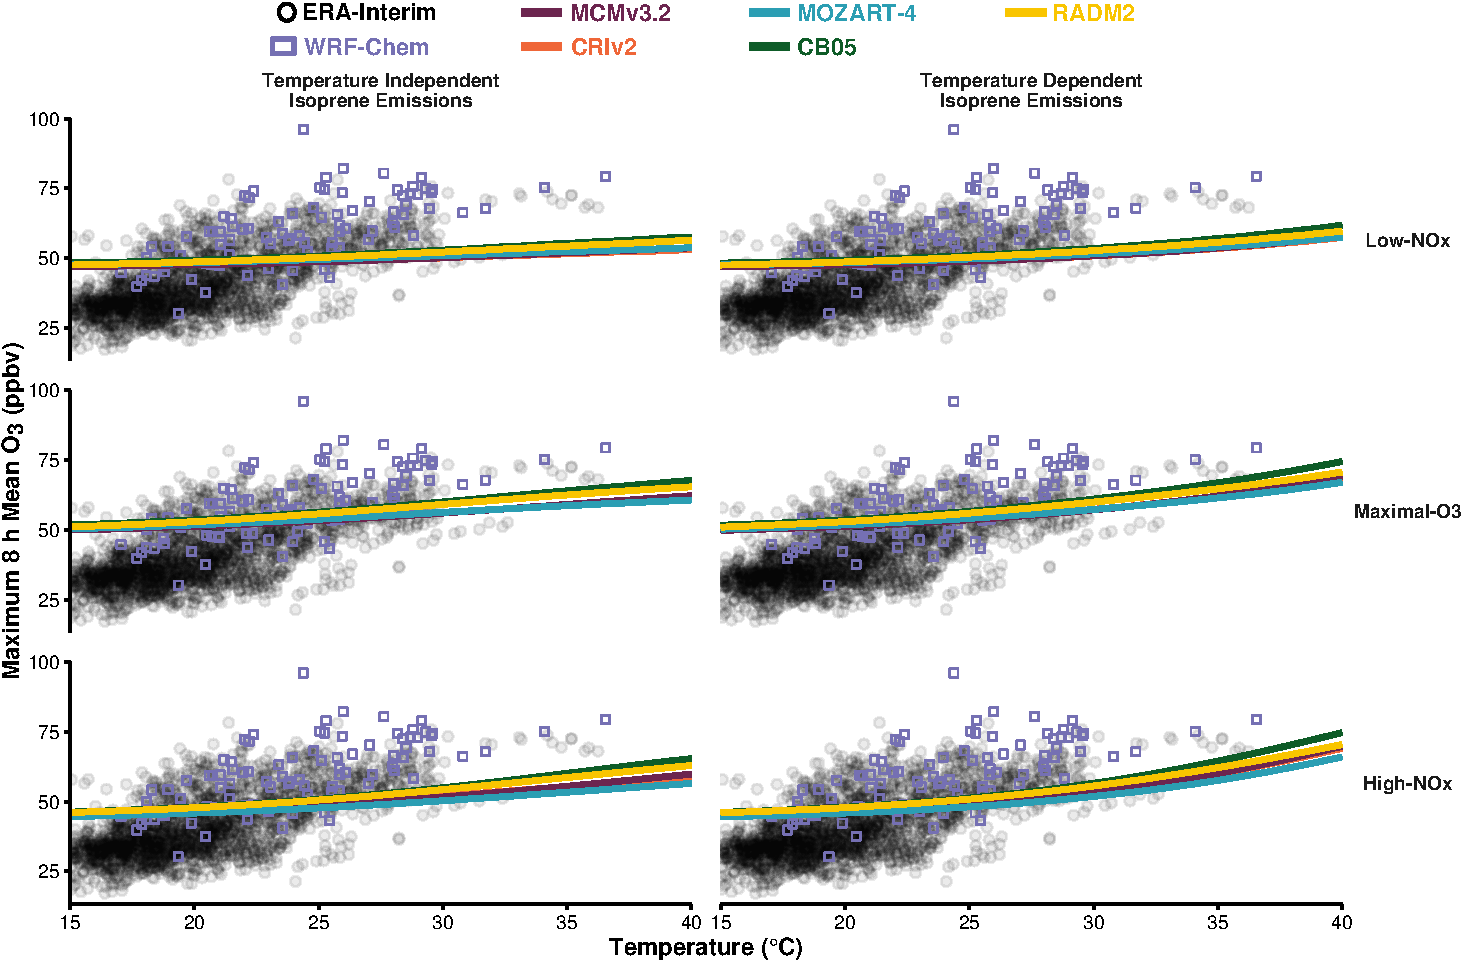
\includegraphics[height=0.43\textheight]{img/Germany_O3-T_ERA_WRF_2007}%
\end{figure}

\begin{table}[t]%
    \centering%
    \caption{Slopes (m$_{\text{O3-T}}$, ppbv per \degree C) of the linear fit to MDA8 values of ozone and temperature correlations in Fig.~\ref{f:comparison}, indicating the increase of MDA8 in ppbv of ozone per \degree C. The slope of the observational data is $2.15$~ppbv/\degree C and the slope of the WRF-Chem output is $2.05$~ppbv/\degree C.}%
    \label{t:mo3-t}%
    \vspace{2mm}
    \scalebox{.78}[.78]{{\renewcommand{\arraystretch}{1.2}
\begin{tabular}{c|c|cc|cc|cc}
	\hline\hline
    \multirow{2}{*}{\textbf{Mechanism}} & \multirow{2}{*}{\textbf{Isoprene Emissions}} & \multicolumn{2}{c|}{\textbf{Low-\chem{NO_x}}} & \multicolumn{2}{c}{\textbf{Maximal-\chem{O_3}}} & \multicolumn{2}{|c}{\textbf{High-\chem{NO_x}}} \\
    & & \textbf{Mixing} & \textbf{No Mixing} & \textbf{Mixing} & \textbf{No Mixing} & \textbf{Mixing} & \textbf{No Mixing} \\
	\hline\hline
	\multirow{2}{*}{MCMv3.2} & Temperature Independent & 0.28 & 1.01 & 0.51 & 1.36 & 0.59 & 0.96 \\ 
    & Temperature Dependent & 0.42 & 1.48 & 0.74 & 2.16 & 0.93 & 2.63 \\ 
	\hline
	\multirow{2}{*}{CRIv2} & Temperature Independent & 0.25 & 0.93 & 0.47 & 1.27 & 0.55 & 0.88 \\ 
    & Temperature Dependent & 0.40 & 1.44 & 0.71 & 2.09 & 0.90 & 2.52 \\ 
	\hline
	\multirow{2}{*}{MOZART-4} & Temperature Independent & 0.25 & 0.97 & 0.44 & 1.21 & 0.49 & 0.59 \\ 
    & Temperature Dependent & 0.38 & 1.43 & 0.65 & 1.98 & 0.81 & 2.05 \\ 
	\hline
	\multirow{2}{*}{CB05} & Temperature Independent & 0.39 & 1.30 & 0.67 & 1.72 & 0.79 & 1.45 \\ 
    & Temperature Dependent & 0.52 & 1.72 & 0.89 & 2.44 & 1.12 & 2.94 \\ 
	\hline
	\multirow{2}{*}{RADM2} & Temperature Independent & 0.37 & 1.31 & 0.61 & 1.64 & 0.70 & 1.28 \\ 
    & Temperature Dependent & 0.48 & 1.68 & 0.79 & 2.22 & 0.97 & 2.49 \\ 
	\hline\hline
\end{tabular}}}
%
    \vspace{-4mm}
\end{table} 

This section compares the results from our idealised box model simulations to real-world observations and model output from a 3D model.
Using the interpolated observations of the maximum daily 8~h mean (MDA8) of ozone from \citet{Schnell:2015} and the meteorological observational data set of the ERA-Interim re-analysis,
\citet{Otero:2016} showed that over the summer (JJA) months, temperature is the main meteorological driver of ozone production over many regions of central Europe.
Model output from the 3D WRF-Chem regional model using MOZART-4 chemistry set-up over the European domain for simulations of the year 2007 from \citet{Mar:2016} was used to further compare the box model simulations to a model including more meteorological processes than our box model.

Figure~\ref{f:comparison} compares the observational and WRF-Chem data from summer 2007 averaged over central and eastern Germany, where summertime ozone values are driven by temperature \citep{Otero:2016}, to the MDA8 values of ozone from the box model simulations for each chemical mechanism (solid lines).
Despite a high bias in simulated ozone in WRF-Chem, the rate of change of ozone with temperature from the WRF-Chem simulations ($2.05$~ppbv/\degree C) is similar to the rate of change of ozone with temperature from the observed data ($2.15$~ppbv/\degree C).
The differences in ozone production between the different chemical mechanisms with the box model are small compared to the spread of the observational and WRF-Chem data.
A temperature-dependent source of isoprene with high-\ce{NO_x} conditions produces the highest ozone-temperature slope, but is still lower than the observed ozone-temperature slope by a factor of two.
In particular, the box model simulations over-predict the ozone values at lower temperatures and under-predict the ozone values at higher temperatures compared to the observed data.

In our simulations, we focused on instantaneous production of ozone from a freshly-emitted source of VOC with mixing of clean air from the free troposphere due to a growing boundary layer.
This box model setup did not consider stagnant atmospheric conditions characteristed by low wind speeds slowing the transport of ozone and its precursors away from sources.
Stagnant conditions have been correlated to high-ozone episodes in the summer over eastern US \citep{Jacob:1993}.

In order to investigate the sensitivity of ozone production to mixing, box model simulations were performed without vertical mixing to approximate stagnant conditions that favour accumulation of secondary VOC oxidation products.
The ozone-temperature relationship obtained with each chemical mechanism, using both a temperature-independent and temperature-dependent source of isoprene emissions and the different \ce{NO_x} conditions are displayed in Fig.~\ref{f:comparison} (dotted lines).
Table~\ref{t:mo3-t} summarises the slopes (m$_{\text{O3-T}}$) of the linear fits of the box model simulations displayed in Fig.~\ref{f:comparison} in ppbv of ozone per \degree C determining the rate of increase of ozone with temperature, for both case: with, and without mixing.

For all chemical mechanisms, the rate of increase of ozone with temperature increased in the box model simulations without mixing.
The m$_{\text{O3-T}}$ calculated from the box model simulations without mixing using a temperature-dependent source of isoprene and with Maximal-\ce{O3} conditions (ranging between $2.0$ and $2.4$~ppbv/\degree C) are very similar to the slopes of the observational and WRF-Chem results ($2.1$ and $2.2$~ppbv/\degree C, respectively).
The differences in m$_{\text{O3-T}}$ when not including mixing in the box model compared to the differences in m$_{\text{O3-T}}$ between chemical mechanisms in Table~\ref{t:mo3-t} show that the ozone-temperature relationship using our box model setup is more sensitive to mixing than the choice of chemical mechanism.

An analysis similar to that presented in Fig.~\ref{f:ozone_budgets} shows no appreciable difference between the cases with and without mixing (not shown).
The chemical production of \ce{O_x} in each chemical mechanism normalised by the chemical loss rate of VOC remains unchanged. 
Furthermore, the supplementary material includes the absolute production and consumption budgets of \ce{O_x} which also show the increased \ce{O_x} production with temperature for the simulations performed without mixing.
From this we conclude that the increased ozone production seen in the box model simulations with reduced mixing is due to enhanced OH reactivity from secondary VOC oxidation products.
